\documentclass[11pt]{report}
\usepackage[pages=some]{background} % package for background
%\usepackage{background} % package for background
\usepackage{graphicx} % package for images
\usepackage{fontspec} % package for fonts
\usepackage[portuguese]{babel} % package for Portuguese language settings (hyphenation, etc.)
\usepackage{helvet} % package for font 'Helvetica'
\usepackage{color} % package for colors
\usepackage{soul} % package for text highlighting
\usepackage{fancyhdr} % package for header and footer formatting
\usepackage{titlesec} % package for chapter name formatting
\usepackage{hyperref} % package for hyperlinks
\usepackage{imakeidx} % package for indices
\usepackage[backend=biber,
            style=authoryear,
            sorting=nyt,
            maxcitenames=2,
            giveninits=true]{biblatex} % package for bibliography
\usepackage[toc]{glossaries} % package for glossaries
\usepackage{tocbibind} % package for toc listing
\usepackage[a4paper, top=2.5cm, bottom=2.5cm, left=3cm, right=3cm]{geometry} % sets page size and margins
\graphicspath{{/images}} % sets images folder
%\RequirePackage{ul-version}
\usepackage{titlesec}
\usepackage{ul-version}
\usepackage{todonotes}  % Para os comandos \todo
\usepackage{graphicx}   % Para incluir imagens
% \usepackage[round]{natbib}  % Remove or comment out this line
\usepackage{pdflscape}
\usepackage{longtable}  % Para tabelas longas que podem quebrar páginas
\usepackage{adjustbox}  % Para redimensionar tabelas


% home background settings
\backgroundsetup{
    scale=1,
    opacity=1,
    angle=0,
    position=current page.center,
    contents={
\includegraphics[width=\paperwidth,height=\paperheight]{images/home_background}}
    %pages=some
}

% hyperlinks setup
\hypersetup{
    linktoc=all,
    colorlinks = true,
    linkcolor={black!50!black},
    citecolor={black!50!black},
    urlcolor={black!80!black}
}

% chapter name formatting
\titleformat{\chapter}[hang]
{\normalfont\huge\bfseries}{\Huge\thechapter \hspace{0.5em}- }{0pt}{\Huge}
\titlespacing*{\chapter}{0pt}{0pt}{20pt}

% header and footer settings
\setlength{\headheight}{18pt} % adjusts head height for header compatibility
\addtolength{\topmargin}{-4.4pt} % adjusts top margin to compensate for change
\fancypagestyle{plain}{
    \pagestyle{fancy}
    \fancyhf{}
    \fancyhead[L]{\large{\textit{Ferramenta de Anotação}}} % sets header
    \fancyfoot[R]{\rule{\textwidth}{0.4pt}\\\thepage}
}

% indice settings
\makeindex
\renewcommand{\contentsname}{Índice} % updates name of the indice page

% bibliography settings
\addbibresource{bibliography.bib}

% glossary entries
\newacronym{lei}{LEI}{Licenciatura em Engenharia Informática}
\newacronym{tfc}{TFC}{Trabalho Final de Curso}
\makeglossaries

% lists settings
\renewcommand{\listfigurename}{Lista de Figuras}
\renewcommand{\listtablename}{Lista de Tabelas}

% font settings
\renewcommand{\familydefault}{\sfdefault} % sets default font family}
\setsansfont{Arial}


% document settings
\title{Ferramenta de Anotação}
\author{Fábio Lopes}
\date{Data}

\DeclareNameAlias{sortname}{family-given}
\DeclareFieldFormat{title}{#1}

\begin{document}
	
    %!TEX root = ./main.tex
\begin{titlepage}
    \BgThispage
    \centering
    \vspace*{7cm}
    
    {\fontsize{50}{1.15}\selectfont Ferramenta de Anotação}
    \vspace{3cm}

    {\fontsize{29}{1.15}\selectfont
        \textbf{Trabalho Final de Curso}\\
    }

    \vspace{1\baselineskip}
    {\fontsize{14}{1.15}\selectfont
        Relatório Final - 3ª Entrega
    }

    \vspace{5.5cm}
    {\fontsize{10}{16}\selectfont
        {Fábio Lopes - a22103261} \\
        {\textbf{Orientador:}} \\
        {Bruno Saraiva} \\
        {\textbf{Co-orientador:}} \\
        {Zuil Filho}

        \vspace{0.3cm}
        Trabalho Final de Curso $|$ LEI $|$ {2024/25}
    }
\end{titlepage}
    %!TEX root = ./main.tex
\thispagestyle{plain}

\vspace*{\fill}

\begin{flushleft}
%\fontfamily{cmr}\selectfont
\rmfamily
{\fontsize{14}{1.15}\selectfont
    \textbf{Direitos de cópia}
}
\vspace{2\baselineskip}

\normalsize{{Ferramenta de Anotação}, Copyright de {Fábio Lopes}, Universidade Lusófona.

A Escola de Comunicação, Arquitectura, Artes e Tecnologias da Informação (ECATI) e a Universidade Lusófona (UL) têm o direito, perpétuo e sem limites geográficos, de arquivar e publicar esta dissertação através de exemplares impressos reproduzidos em papel ou de forma digital, ou por qualquer outro meio conhecido ou que venha a ser inventado, e de a divulgar através de repositórios científicos e de admitir a sua cópia e distribuição com objectivos educacionais ou de investigação, não comerciais, desde que seja dado crédito ao autor e editor.}\\
Este documento foi gerado com o processador (pdf/Xe/Lua)\LaTeX\ e o modelo \href{https://github.com/joaomlourenco/novathesis}{ULThesis} (v\ulthesisversion)~\cite{ulthesis-manual}.
\end{flushleft}
    %\input{agradecimentos}
    %!TEX root = ./main.tex
\chapter*{Resumo}
\addcontentsline{toc}{chapter}{Resumo}

Este trabalho apresenta o desenvolvimento de uma ferramenta de anotação que implementa um Módulo de Chat Disentanglement especializado, concebido para apoiar a criação de datasets anotados para investigação em conversation disentanglement. O módulo disponibiliza uma interface de utilizador onde os anotadores podem identificar e marcar diferentes threads de conversa que ocorrem simultaneamente em dados de chatrooms. O Chat Disentanglement, conforme descrito por \textcite{elsner2010disentangling}, é a tarefa de separar múltiplas conversas concorrentes num único canal de comunicação. A nossa ferramenta de anotação foca-se em fornecer uma experiência de utilizador intuitiva e fácil para minimizar erros de anotação, e será utilizada pelo AISIC Lab (Artificial Intelligence and Social Interaction and Complexity) para criar datasets anotados de conversas de chatrooms, que podem depois ser utilizados por investigadores e anotadores para estudar e desenvolver soluções automatizadas de disentanglement.

    %!TEX root = ./main.tex
\chapter*{Abstract}
\addcontentsline{toc}{chapter}{Abstract}

This work presents the development of an annotation tool that implements a specialized Chat Disentanglement Module, designed to support the creation of annotated datasets for conversation disentanglement research. The module provides a user interface where annotators can identify and mark different conversation threads occurring simultaneously in chatroom data. Chat disentanglement, as described by \textcite{elsner2010disentangling}, is the task of separating multiple concurrent conversations in a single communication channel. Our annotation tool focuses on providing an intuitive and easy user experience to minimize annotation errors, and will be used by the AISIC Lab (Artificial Intelligence and Social Interaction and Complexity) to create annotated datasets of chatroom conversations, which can then be utilized by researchers and annotators to study and develop automated disentanglement solutions.
    
    \tableofcontents
    \listoffigures
    \listoftables
    \printglossary[type=\acronymtype,title={Lista de Siglas e Acrónimos}]
    
    % Chapters
    \chapter{Introdução}

No contexto atual do AISIC LAB - Artificial Intelligence, Social Interaction and Complexity, pertencente ao CICANT da Universidade Lusófona, surge a necessidade de desenvolver uma infraestrutura modular para anotação de dados, com particular incidência em aplicações de Processamento de Linguagem Natural (NLP). Este projeto visa responder aos desafios específicos encontrados no laboratório, nomeadamente na análise e processamento de interações em ambientes de chat.

\section{Enquadramento}

A anotação de dados é um processo fundamental no treino de modelos de Machine Learning, particularmente importante em aplicações de NLP. Este processo envolve a atribuição sistemática de etiquetas, categorias ou metadados a conjuntos de dados não processados, permitindo que os algoritmos aprendam padrões e características específicas. Os dados anotados funcionam como referência fundamental, possibilitando o treino de modelos para reconhecer e classificar informações de forma precisa.

\section{Motivação e Identificação do Problema}

A motivação principal deste projeto emerge das necessidades específicas identificadas no AISIC LAB, onde a análise de mensagens em grupos de chat, requer ferramentas especializadas de anotação. 
Através de análises preliminares e feedback dos investigadores, identificámos três desafios fundamentais:

\begin{enumerate}
    \item \textbf{Complexidade das Tarefas de Anotação}:
    \begin{itemize}
        \item Necessidade de suporte a diferentes tipos de anotação
        \item Gestão de múltiplos anotadores e controle de qualidade
        \item Requisitos específicos para diferentes domínios de aplicação
    \end{itemize}

    \item \textbf{Limitações das Ferramentas Existentes}:
    \begin{itemize}
        \item Ferramentas estabelecidas como o BRAT\footnote{\cite{brat-repo,brat-about}} apresentam limitações tecnológicas e falta de evolução
        \item Soluções atuais como o Doccano\footnote{\cite{doccano-repo,doccano-docs}}, que utiliza Django como framework backend, impõem uma estrutura mais rígida, o que limita a capacidade de realizar adaptações específicas às necessidades do projeto.
        \item Necessidade de maior flexibilidade na modelação de dados e lógica aplicacional
        \item Dificuldade de integração com fluxos de trabalho existentes e específicos
    \end{itemize}

    \item \textbf{Necessidade de Integração Completa do Workflow}:
    \begin{itemize}
        \item Gestão integrada das fases pré-anotação, anotação e pós-anotação
        \item Necessidade de implementação de métricas e análises específicas
        \item Suporte a fluxos customizados de processamento de dados
        \item Integração com pipelines de NLP e análise de dados existentes
    \end{itemize}
\end{enumerate}

A decisão de desenvolver uma solução dedicada, em vez de adaptar ferramentas existentes, fundamenta-se na necessidade de maior controlo sobre todo o processo de anotação. Esta abordagem permite-nos focar no desenvolvimento de funcionalidades específicas para o nosso caso de uso principal - a tarefa de disentanglement de chat - garantindo a flexibilidade necessária para implementar workflows customizados de pré-processamento, anotação e análise posterior dos dados.

\section{Objetivos}

O projeto tem como objetivos principais:

\begin{enumerate}
    \item \textbf{Desenvolvimento de Infraestrutura Modular}:
    \begin{itemize}
        \item Criar uma plataforma flexível e extensível para anotação de dados
        \item Implementar sistema de plugins para diferentes tipos de tarefas
        \item Desenvolver interfaces programáticas (APIs) para integração com outros sistemas
    \end{itemize}

    \item \textbf{Automação e Controlo de Qualidade}:
    \begin{itemize}
        \item Implementar distribuição automática de tarefas
        \item Desenvolver sistema robusto de métricas e validações
        \item Criar mecanismos de controle de qualidade e consistência
    \end{itemize}

    \item \textbf{Suporte a Múltiplos Domínios}:
    \begin{itemize}
        \item Permitir configuração de diferentes esquemas de anotação
        \item Implementar suporte para diversos tipos de dados
        \item Facilitar a extensão para novos casos de uso
    \end{itemize}

    \item \textbf{Usabilidade e Produtividade}:
    \begin{itemize}
        \item Desenvolver interfaces intuitivas para anotadores
        \item Implementar ferramentas de gestão e monitoramento
        \item Criar documentação abrangente e guias de utilização
    \end{itemize}
\end{enumerate}

\section{Estrutura do Documento}

Este documento está organizado da seguinte forma:

\begin{itemize}
    \item \textbf{Capítulo 2 - Pertinência e Viabilidade}: Apresenta análise detalhada do contexto atual, comparação com soluções existentes e identificação de oportunidades de inovação.

    \item \textbf{Capítulo 3 - Especificação e Modelação}: Detalha requisitos funcionais e não-funcionais, casos de uso e a modelação da solução proposta.

    \item \textbf{Capítulo 4 - Solução Proposta}: Descreve a arquitetura, tecnologias utilizadas e os componentes principais da solução em desenvolvimento.

    \item \textbf{Capítulo 5 - Testes e Validação}: Apresenta o plano delineado para testar e validar a ferramenta, incluindo a metodologia, cenários e métricas de avaliação.

    \item \textbf{Capítulo 6 - Método e Planeamento}: Detalha a abordagem metodológica seguida e analisa o progresso do desenvolvimento face ao planeamento.

    \item \textbf{Capítulo 7 - Resultados}: (A desenvolver) Discutirá os resultados obtidos nos testes e avaliará o cumprimento dos objetivos.

    \item \textbf{Capítulo 8 - Conclusão}: (A desenvolver) Sintetizará as contribuições do trabalho e apresentará perspetivas futuras.
\end{itemize}

Os anexos poderão incluir documentação técnica adicional, guiões de teste ou outros materiais de suporte relevantes.

    \chapter{Pertinência e Viabilidade}

\section{Pertinência}
O desenvolvimento de uma ferramenta modular para anotação de dados surge como resposta a uma necessidade crítica no campo do processamento de linguagem natural (NLP). A pertinência desta solução é evidenciada por múltiplos fatores.

O AISIC LAB, validou a necessidade desta ferramenta através de feedback direto dos anotadores sobre as limitações das ferramentas atuais, bem como através da avaliação dos investigadores sobre o impacto na qualidade dos dados e análise das necessidades específicas de projetos em andamento.

O desenvolvimento desta ferramenta promete uma redução significativa no tempo de anotação, além de proporcionar uma melhoria substancial na qualidade e consistência dos dados anotados. A solução também facilita a colaboração entre anotadores e oferece suporte flexível a múltiplos tipos de tarefas de anotação, adaptando-se às necessidades específicas de cada projeto.

\section{Viabilidade}
A implementação da solução demonstra-se viável em múltiplas dimensões. Do ponto de vista técnico, a experiência prévia com um protótipo funcional em React, combinada com a disponibilidade de frameworks modernos para desenvolvimento, fornece uma base sólida para o projeto. A arquitetura modular planeada permite um desenvolvimento incremental e sustentável, aproveitando a infraestrutura existente para deployment.

Quanto à viabilidade económica, o projeto beneficia de um baixo custo de desenvolvimento inicial, principalmente devido à utilização de tecnologias open-source. Além disso, apresenta potencial para comercialização futura e promete uma redução significativa nos custos operacionais relacionados à anotação de dados.

A aceitação social do projeto é confirmada pelo feedback positivo dos utilizadores finais e pelo forte alinhamento com as necessidades do departamento. O potencial de aplicação em outros contextos académicos e a contribuição significativa para a pesquisa em NLP reforçam sua relevância no ambiente académico e científico.

\section{Análise Comparativa com Soluções Existentes}

\subsection{Soluções Existentes}

\subsubsection{Doccano}
O Doccano é uma plataforma open-source para anotação de dados em NLP. A ferramenta oferece suporte a múltiplos tipos de anotação e possui uma arquitetura modular que permite extensões dentro da sua estrutura.

\subsubsection{BRAT}
O BRAT é uma ferramenta estabelecida para anotação de texto, com foco em simplicidade e interface intuitiva. Apesar de sua maturidade, apresenta limitações em termos de extensibilidade e modernização.

\subsection{Análise de Benchmarking}

A Tabela~\ref{tab:tech-comparison} apresenta uma comparação detalhada das características técnicas de cada solução. Esta análise permitiu identificar pontos fortes e limitações de cada ferramenta, orientando o desenvolvimento da solução proposta.

\section{Proposta de Inovação e Mais-Valias}
A solução desenvolvida foca-se especificamente nas necessidades de anotação para a tarefa dedisentanglement de chat nesta fase inicial, permitindo uma implementação direta e eficiente deste tipo de tarefa. A abordagem modular facilita a adaptação para diferentes necessidades de anotação, com o objetivo futuro de suportar múltiplos tipos de tarefas de anotação, mantendo a simplicidade de uso.

\section{Identificação de Oportunidade de Negócio}
O projeto apresenta potencial para aplicação em contextos acadêmicos e de pesquisa, especialmente em grupos que trabalham com processamento de linguagem natural. A capacidade de adaptação para diferentes tipos de anotação permite atender necessidades específicas de diversos projetos de pesquisa.

\clearpage
\begin{table}[p]
\setlength{\footnotesep}{15pt}
\begin{minipage}{\textwidth}
\centering
\begin{tabular}{|l|p{0.25\textwidth}|p{0.25\textwidth}|p{0.25\textwidth}|}
\hline
\textbf{Solução} & \textbf{BRAT\protect\footnotemark[1]} & \textbf{Doccano\protect\footnotemark[2]} & \textbf{Solução Proposta} \\
\hline
Frontend & jQuery 1.7.1 + jQuery UI, SVG para visualização, JavaScript vanilla, XHTML templates & Nuxt.js framework, Vue.js (implícito via Nuxt), Modern JavaScript/TypeScript & React 18, TypeScript, Componentes funcionais, Hooks customizados \\
\hline
Backend & Python 2.5+, CGI/FastCGI, Bibliotecas JSON & Python 3.8+, Django 4.0+, REST API architecture & Express.js (protótipo), Migração planeada para Flask/FastAPI \\
\hline
Formato de Anotação & Arquivos .ann para anotações, Arquivos .txt para texto, JSON para comunicação & REST API endpoints, JSON para comunicação & REST API para comunicação e configuração, Suporte planeado para múltiplos formatos \\
\hline
Dados & Sistema de arquivos, Estrutura em diretórios, Sem banco de dados & Database (Django ORM), Suporte a PostgreSQL & Suporte planeado para múltiplos formatos (CSV, TXT, JSON, Markdown), Cache local opcional via SQLite \\
\hline
Deployment & Apache/Lighttpd com CGI, Standalone Python server & Docker containers, Docker Compose support, Production/Development configs & Container Docker único, Setup simplificado \\
\hline
Extensibilidade & Sistema via arquivos .conf, Arquitetura modular, Plugins jQuery & Modular Django architecture, REST API extensibility, Frontend component system & Componentes React modulares, Hooks customizáveis, API extensível \\
\hline
Estado de Manutenção & Última atualização ~2012, Tecnologias desatualizadas, Projeto inativo & Projeto ativo, Tecnologias modernas, Atualizações regulares & Em desenvolvimento ativo, Stack moderna, Iterações frequentes \\
\hline
Documentação & README detalhado, Exemplos incluídos, Tutoriais no código & Documentação estruturada, Guias de desenvolvimento, Diagramas de arquitetura & Documentação focada, Exemplos práticos, Guias de desenvolvimento \\
\hline
Requisitos Sistema & Python 2.5+, Servidor Web com CGI, Browser com SVG & Python 3.8+, Docker (recomendado), Node.js para desenvolvimento & Node.js 18+ (atual), Python 3.x (planeado), Navegador moderno, Docker (opcional) \\
\hline
Segurança & Autenticação básica, Controle via arquivo & Django authentication, Modern security practices & Autenticação básica baseada em roles (administrador/anotador) \\
\hline
\end{tabular}
\caption{Comparação técnica detalhada das soluções}
\label{tab:tech-comparison}

\footnotetext[1]{\cite{brat-repo,brat-about}}
\footnotetext[2]{\cite{doccano-repo,doccano-docs}}
\end{minipage}
\end{table}


    \chapter{Especificação e Modelação}
\label{cha:especificacao_modelacao}

Neste capítulo, são detalhadas as especificações técnicas da solução desenvolvida. A análise de requisitos é apresentada em primeiro lugar, seguida pela modelação da arquitetura, da base de dados e da API, que em conjunto definem a estrutura e o comportamento do sistema.

\section{Análise de Requisitos}

A tabela seguinte resume os requisitos funcionais (RF) e não-funcionais (RNF) identificados para o projeto, juntamente com o estado final da sua implementação.

% Tabela de Requisitos atualizada
\begin{table}[h!]
    \centering
    \begin{tabular}{|p{0.1\textwidth}|p{0.5\textwidth}|p{0.15\textwidth}|p{0.15\textwidth}|}
        \hline
        \textbf{ID} & \textbf{Descrição} & \textbf{Estado} & \textbf{Notas} \\
        \hline
        \multicolumn{4}{|c|}{\textbf{Requisitos Funcionais}} \\
        \hline
        RF1 & Suporte à importação de dados (CSV, JSON) & Cumprido & Implementada importação de mensagens via CSV e anotações via JSON. \\
        \hline
        RF2 & Organização de dados por projetos & Cumprido & Estrutura central da aplicação. \\
        \hline
        RF3 & Exportação dos dados anotados (JSON) & Cumprido & Funcionalidade de exportação por sala de chat implementada. \\
        \hline
        RF4 & Interface de utilizador clara e funcional & Cumprido & Interface React desenvolvida com foco na usabilidade para anotação. \\
        \hline
        RF5 & Suporte a múltiplos anotadores por projeto & Cumprido & Sistema de atribuição de utilizadores a projetos. \\
        \hline
        RF6 & Gestão de atribuição de tarefas & Cumprido & Administradores podem atribuir/remover utilizadores de projetos. \\
        \hline
        RF7 & Interface especializada para chat disentanglement & Cumprido & Ecrã de anotação dedicado com gestão de threads. \\
        \hline
        RF8 & Sistema de tagging para classificação em threads & Cumprido & Funcionalidade nuclear da anotação. \\
        \hline
        RF9 & Visualização sequencial das mensagens & Cumprido & A sala de chat apresenta as mensagens por ordem. \\
        \hline
        RF10 & Armazenamento para cálculo de métricas & Cumprido & O modelo de dados permite o cálculo de IAA. \\
        \hline
        RF11 & Autenticação de utilizadores & Cumprido & Implementado com JWT (access e refresh tokens). \\
        \hline
        RF12 & Definição de roles (admin/anotador) & Cumprido & O modelo `User` contém o campo `is\_admin`. \\
        \hline
        RF13 & Controlo de acesso baseado em permissões & Cumprido & Endpoints da API protegidos com base no role. \\
        \hline
        \multicolumn{4}{|c|}{\textbf{Requisitos Não Funcionais}} \\
        \hline
        RNF1 & Tempo de resposta adequado & Cumprido & A API responde rapidamente a pedidos interactivos. \\
        \hline
        RNF2 & Processamento eficiente para múltiplos utilizadores & Parcialmente & A arquitetura suporta-o, mas não foram feitos testes de carga formais. \\
        \hline
        RNF3 & Interface responsiva & Parcialmente & O design é funcional mas não foi totalmente otimizado para todos os tamanhos de ecrã. \\
        \hline
        RNF4 & Feedback visual claro & Cumprido & A interface React fornece feedback sobre o estado (loading, error, success). \\
        \hline
        RNF5 & Interface simples e intuitiva & Cumprido & O design focou-se na simplicidade para a tarefa de anotação. \\
        \hline
        RNF6 & Backup automático de anotações & Não Cumprido & Não implementado. Requer uma solução de infraestrutura (e.g., cron jobs na base de dados). \\
        \hline
        RNF7 & Logging de atividades críticas & Parcialmente & O backend utiliza logging básico, mas não um sistema de logging estruturado e exaustivo. \\
        \hline
    \end{tabular}
    \caption{Tabela de Requisitos e Estado de Implementação.}
    \label{tab:requisitos}
\end{table}

\section{Modelação da Solução}

A modelação da solução foi um processo iterativo que resultou numa arquitetura de três camadas, um modelo de dados relacional robusto e uma API RESTful bem definida.

\subsection{Arquitetura da Solução}

A plataforma segue uma arquitetura cliente-servidor moderna e desacoplada, composta por dois componentes principais:

\begin{itemize}
    \item \textbf{Frontend (Cliente):} Uma Single-Page Application (SPA) desenvolvida com a biblioteca \textbf{React}. É responsável exclusivamente pela apresentação da interface do utilizador e pela gestão do estado local da UI. Toda a lógica de negócio e manipulação de dados é delegada ao backend através de chamadas à API.
    \item \textbf{Backend (Servidor):} Uma API RESTful desenvolvida com a framework \textbf{FastAPI} (Python). É responsável por toda a lógica de negócio, incluindo a autenticação de utilizadores, controlo de permissões, operações na base de dados (CRUD) e cálculos de métricas como o IAA.
\end{itemize}
Esta separação estrita de responsabilidades (`separation of concerns`) garante uma maior manutenibilidade, escalabilidade e a possibilidade de desenvolver e testar os dois componentes de forma independente.

\subsection{Modelo de Dados}

O coração do backend é o seu modelo de dados relacional, implementado com \textbf{SQLAlchemy} como ORM (Object-Relational Mapper), que mapeia as classes Python para tabelas numa base de dados SQL. A Figura~\ref{fig:modelo-er} apresenta o Diagrama de Entidade-Relação (ERD) final do sistema.

As entidades centrais do modelo são:
\begin{itemize}
    \item \textbf{User, Project, e ProjectAssignment:} que em conjunto gerem os utilizadores e as suas permissões de acesso aos diferentes projetos.
    \item \textbf{ChatRoom e ChatMessage:} que estruturam os dados a serem anotados.
    \item \textbf{Annotation:} a tabela principal que armazena a ligação entre uma mensagem, um anotador e um \textit{thread}, sendo a base para toda a análise posterior.
\end{itemize}
A utilização do SQLAlchemy e do Alembic para migrações de base de dados permitiu uma evolução estruturada do esquema ao longo do desenvolvimento do projeto.

\subsection{API RESTful}

A comunicação entre o frontend e o backend é realizada através de uma API RESTful. A API expõe um conjunto de endpoints para todas as operações necessárias, desde a autenticação até ao cálculo de métricas. A API está documentada seguindo o standard OpenAPI, o que facilita a sua exploração e integração.

Os endpoints estão logicamente agrupados por responsabilidade:
\begin{itemize}
    \item \textbf{Auth:} Gestão de autenticação e tokens.
    \item \textbf{Projects:} Operações de utilizador normal sobre projetos e salas de chat.
    \item \textbf{Annotations:} Criação e gestão de anotações.
    \item \textbf{Admin:} Operações de administração, incluindo importação/exportação e cálculo de IAA.
\end{itemize}

\section{Protótipos de Interface}

\subsection{Mapa de Navegação}

A estrutura de navegação da plataforma está idealizada para adaptar-se aos diferentes perfis de utilizador. O sistema prevê um portal de login onde após autenticação, os utilizadores terão acesso a um dashboard principal, que funcionará como ponto central de acesso às diversas funcionalidades da plataforma. A estrutura completa do mapa de navegação pode ser visualizada na Figura~\ref{fig:mapa-navegacao}, que foi modificada para ocupar uma página inteira em landscape.

A ferramenta de anotação será estruturada de forma modular, onde o dashboard principal permitirá acesso aos vários módulos disponíveis. Numa primeira fase, o módulo de disentanglement será o unico modulo desta arquitetura modular, no entanto o objetico da ferramenta de anotação será de acomodar mais módulos no futuro.

\subsection{Principais Interfaces}

\subsubsection{Portal de Entrada}
O acesso à plataforma é controlado através de um portal de autenticação minimalista. Esta decisão de design visa garantir a integridade dos dados e a atribuição correta das tarefas de anotação, sendo o login obrigatório para qualquer interação com os dados do sistema.

\subsubsection{Dashboard Principal}
Após autenticação, o utilizador acede a um dashboard que apresenta uma visão geral da plataforma. Este componente central adapta-se dinamicamente ao perfil do utilizador (administrador ou anotador), apresentando as funcionalidades relevantes e o estado atual das tarefas atribuídas.

\subsubsection{Módulo de Disentanglement}
O primeiro módulo implementado na plataforma foca-se na tarefa de disentanglement de chat, apresentando duas visões distintas:

\paragraph{Visão do Anotador}
Para os anotadores, a interface apresenta:
\begin{itemize}
    \item Lista das chatrooms atribuídas automaticamente pelo sistema
    \item Interface de anotação com visualização sequencial das mensagens
    \item Sistema intuitivo de tagging para classificação de threads
    \item Indicadores de progresso da tarefa
    \item Mecanismos de validação em tempo real
\end{itemize}

\paragraph{Visão do Administrador}
Os administradores têm acesso a funcionalidades adicionais:
\begin{itemize}
    \item Gestão completa dos datasets
    \item Monitorização do progresso dos anotadores
    \item Visualização de métricas e estatísticas
    \item Configuração da distribuição automática de tarefas
\end{itemize}

\subsubsection{Interface de Anotação}
O componente central do módulo de disentanglement é a interface de anotação, que foi projetada para maximizar a eficiência do processo de anotação. Cada chatroom é apresentada como uma sequência temporal de mensagens, onde o anotador pode facilmente:
\begin{itemize}
    \item Visualizar o contexto completo da conversa
    \item Criar e atribuir tags de thread às mensagens
    \item Acompanhar o progresso da anotação em tempo real
    \item Navegar eficientemente entre diferentes chatrooms
\end{itemize}

O sistema mantém um salvamento automático do progresso, permitindo que os anotadores retomem seu trabalho de forma seamless em qualquer momento.


\begin{figure}[p]
    \centering
    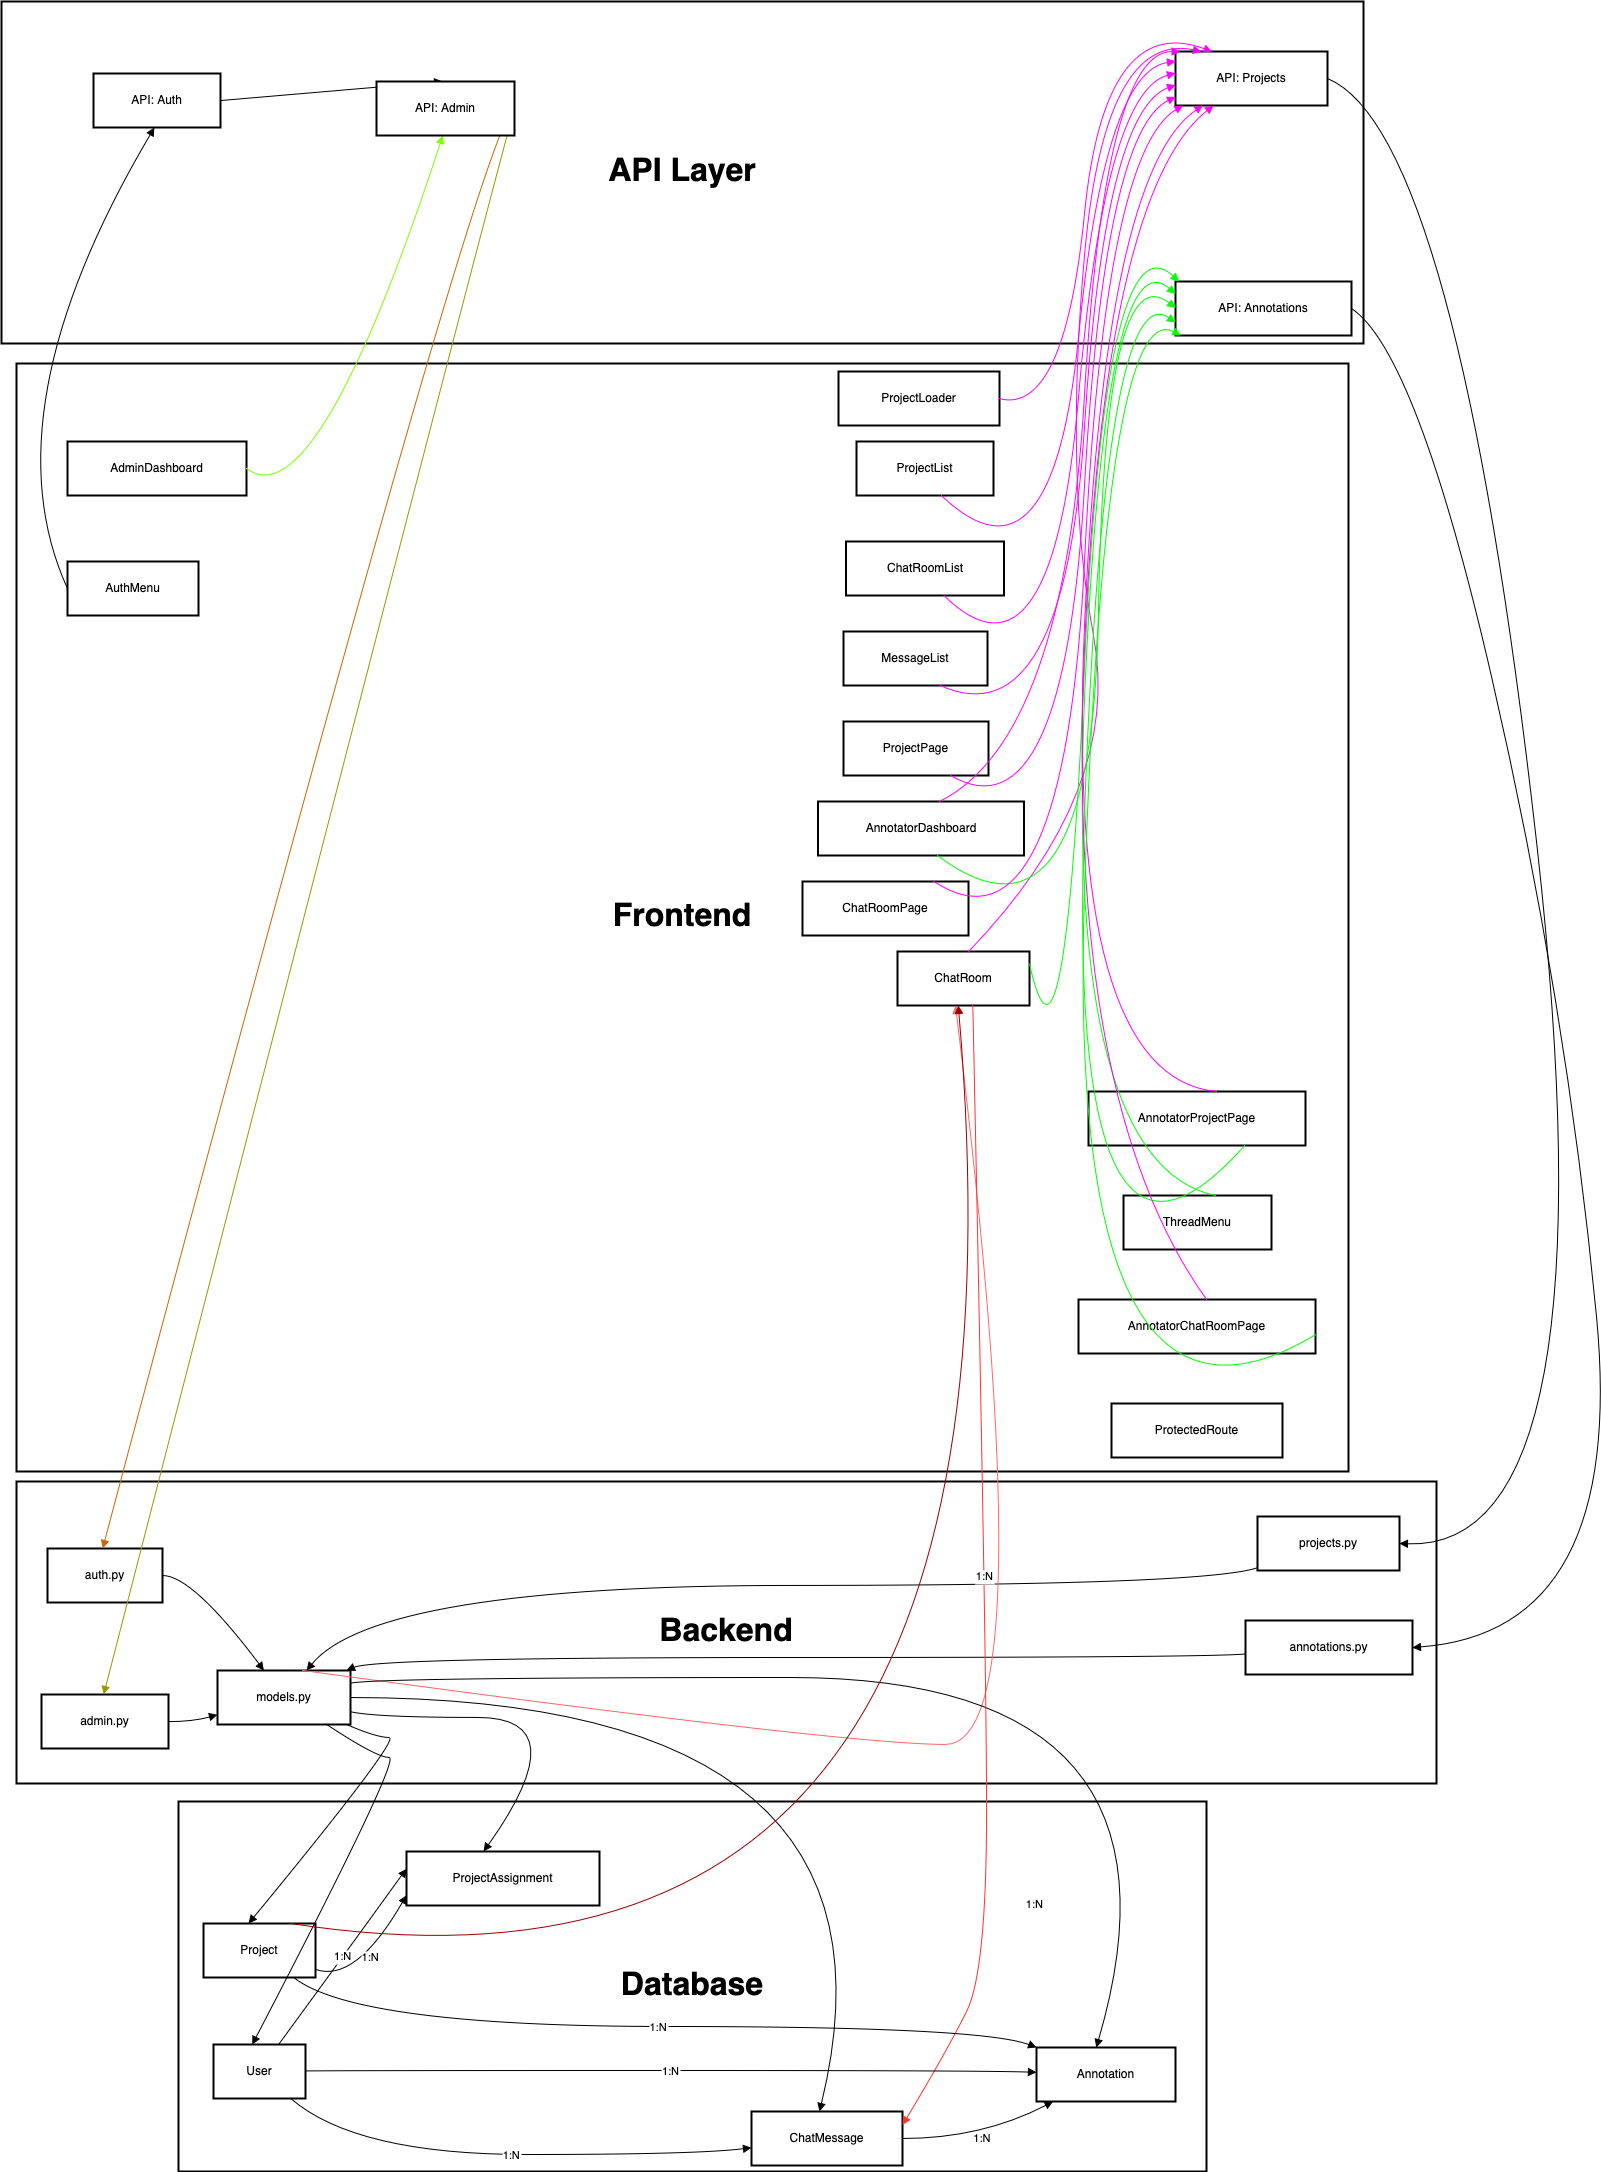
\includegraphics[width=0.95\textwidth,height=0.95\textheight,keepaspectratio]{images/2A-ERT-B.drawio.png}
    \caption{Modelo de Entidade-Relação final do Sistema.}
    \label{fig:modelo-er}
\end{figure}

\begin{landscape}
    \begin{figure}[p]
        \centering
        \makebox[\textwidth][c]{%
            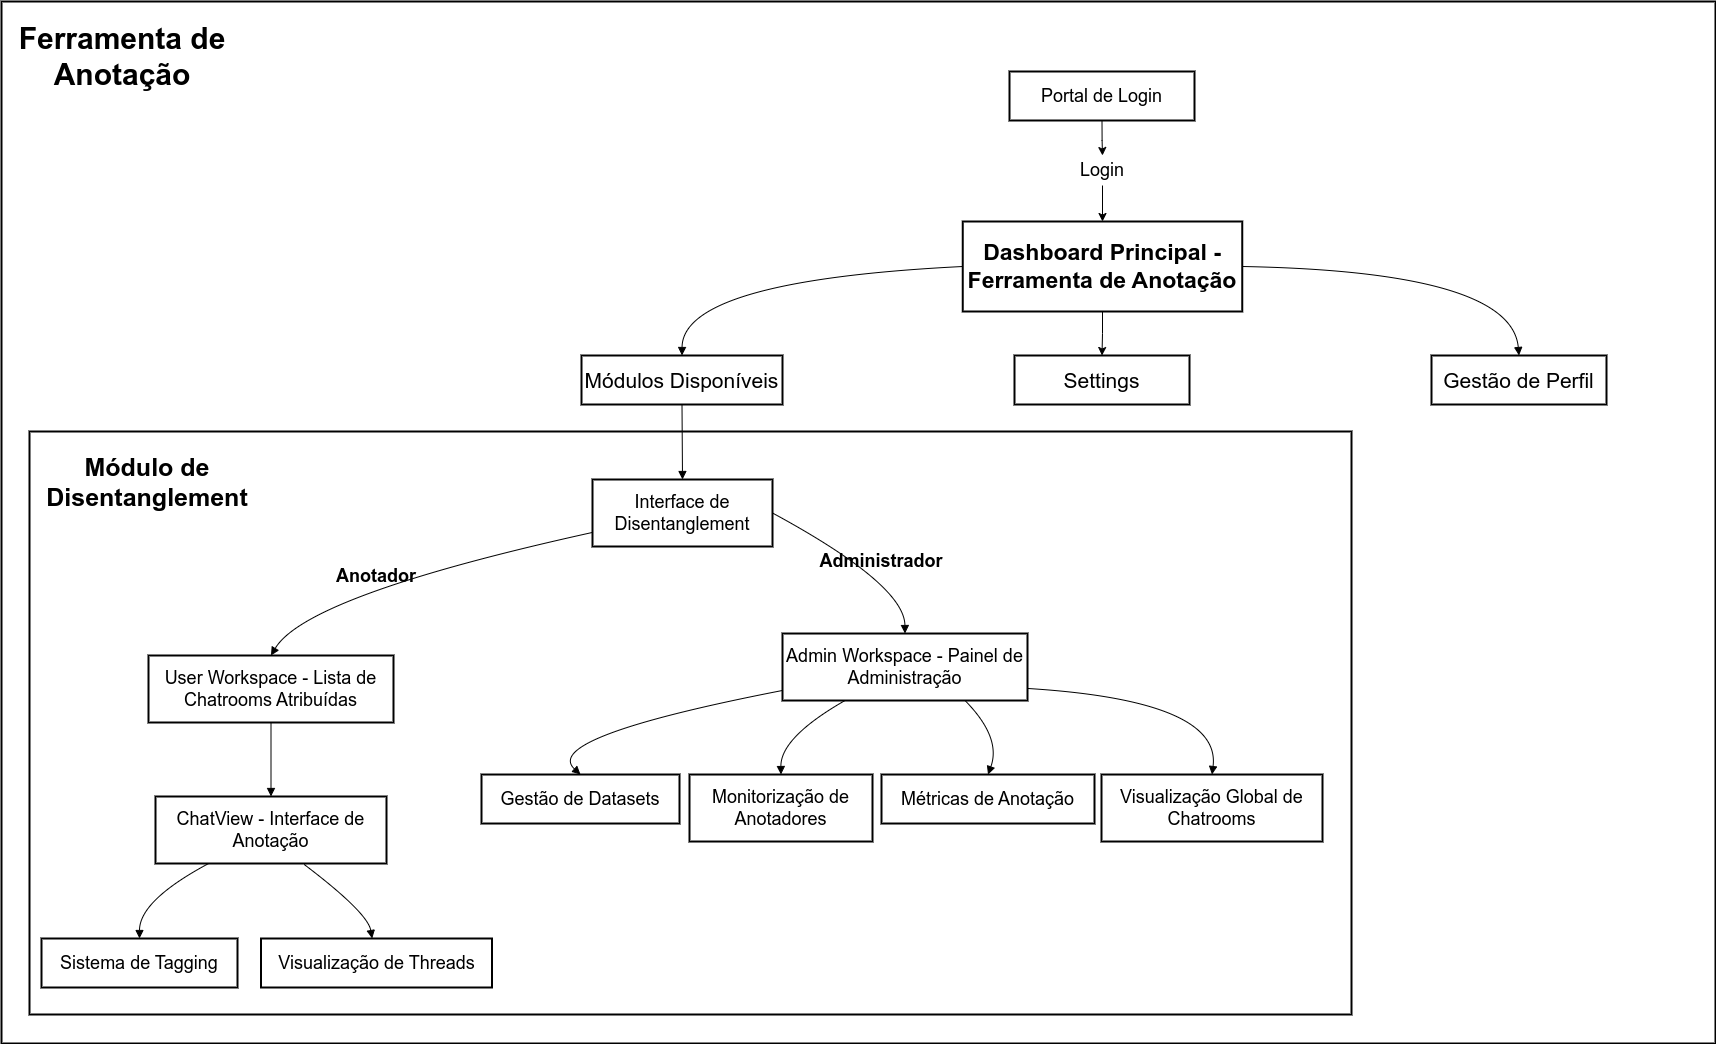
\includegraphics[width=0.8\paperheight, angle=0, keepaspectratio]{images/mapaDeNavegacaoSistema.drawio.png}
        }
        \caption{Mapa de Navegação do Sistema.}
        \label{fig:mapa-navegacao}
    \end{figure}
\end{landscape}
    \chapter{Solução Proposta}
\label{cha:solucao_proposta}

Este capítulo detalha a solução técnica implementada para responder aos requisitos especificados. A apresentação abrange a arquitetura global do sistema, as tecnologias e ferramentas selecionadas para o seu desenvolvimento, e uma descrição dos principais componentes do frontend e do backend.

\section{Arquitetura da Solução}

A plataforma foi desenhada seguindo uma \textbf{arquitetura cliente-servidor desacoplada}, uma abordagem moderna que promove a separação de responsabilidades, a escalabilidade e a manutenibilidade. A solução é composta por dois sistemas independentes que comunicam através de uma API bem definida.

\begin{itemize}
    \item \textbf{Frontend (Cliente):} Uma \textit{Single-Page Application} (SPA) desenvolvida com a biblioteca \textbf{React}. A sua única responsabilidade é renderizar a interface do utilizador (UI) e gerir o estado da interação do utilizador. Toda a lógica de negócio, processamento de dados e autenticação são delegados ao backend através de chamadas a uma API RESTful. Esta abordagem de "cliente puro" garante que o frontend permanece focado na experiência do utilizador.

    \item \textbf{Backend (Servidor):} Um servidor de API RESTful desenvolvido com a framework \textbf{FastAPI} em Python. Este componente é o cérebro da aplicação, responsável por:
    \begin{itemize}
        \item Implementar toda a lógica de negócio.
        \item Gerir a autenticação e autorização de utilizadores.
        \item Executar todas as operações de base de dados (CRUD - Create, Read, Update, Delete).
        \item Realizar os cálculos computacionalmente intensivos, como o Inter-Annotator Agreement (IAA).
    \end{itemize}
\end{itemize}

A comunicação entre os dois componentes é feita exclusivamente através de requisições HTTP, com os dados a serem trocados no formato JSON.
% TODO: Incluir um diagrama de arquitetura de alto nível que mostre os dois componentes (React App, FastAPI App), a base de dados, e o fluxo de comunicação via API REST.

\section{Tecnologias e Ferramentas Utilizadas}

A seleção de tecnologias foi guiada por critérios de performance, maturidade, ecossistema e adequação aos requisitos do projeto. A Tabela~\ref{tab:tecnologias_utilizadas} resume as escolhas feitas.

\begin{table}[h!]
    \centering
    \begin{tabular}{|l|l|p{0.5\textwidth}|}
        \hline
        \textbf{Componente} & \textbf{Tecnologia/Ferramenta} & \textbf{Justificação} \\
        \hline
        \textbf{Frontend} & React 18 & Framework líder para SPAs, com um vasto ecossistema e gestão de estado eficiente através de Hooks e Context API. \\
        & JavaScript (ES6+) & Linguagem padrão para desenvolvimento web. \\
        & Axios & Cliente HTTP para realizar as chamadas à API RESTful de forma fiável e com gestão de intercetores. \\
        & CSS3 & Estilização dos componentes para uma interface limpa e funcional. \\
        \hline
        \textbf{Backend} & Python 3.11 & Linguagem robusta com um forte ecossistema para ciência de dados e desenvolvimento web. \\
        & FastAPI & Framework web de alta performance com validação de dados automática e geração de documentação OpenAPI. \\
        & SQLAlchemy & O principal ORM para Python, permitindo uma interação segura e abstrata com a base de dados. \\
        & Alembic & Ferramenta para a gestão de migrações de esquema da base de dados. \\
        & Pydantic & Biblioteca para validação de dados, utilizada pelo FastAPI para garantir a integridade dos dados. \\
        & SciPy & Biblioteca para computação científica, utilizada para o cálculo do IAA (Algoritmo Húngaro). \\
        & python-jose, passlib & Bibliotecas para a gestão de JWTs e hashing de passwords, garantindo a segurança. \\
        \hline
        \textbf{Base de Dados} & PostgreSQL & SGBD relacional robusto e pronto para produção. \\
        & SQLite & SGBD leve e baseado em ficheiro, ideal para desenvolvimento e testes locais. \\
        \hline
        \textbf{DevOps} & Docker & Plataforma de contentorização para criar ambientes de desenvolvimento e produção consistentes. \\
        \hline
    \end{tabular}
    \caption{Tecnologias e Ferramentas Utilizadas na Solução}
    \label{tab:tecnologias_utilizadas}
\end{table}

\section{Componentes da Solução}

\subsection{Frontend}

O frontend foi estruturado para ser modular e de fácil manutenção, seguindo as melhores práticas do React.

\begin{itemize}
    \item \textbf{Componentes de Página:} Componentes de alto nível que representam uma vista completa (e.g., \texttt{AdminDashboard.js}, \texttt{AnnotatorChatRoomPage.js}). São estes componentes que contêm a lógica de \textit{data-fetching}, chamando a API para obter os dados necessários.
    \item \textbf{Componentes de UI:} Componentes mais pequenos e reutilizáveis (e.g., \texttt{MessageBubble.js}, \texttt{ProjectCard.js}) que são puramente presentacionais e recebem dados via \textit{props}.
    \item \textbf{Gestão de API (\texttt{/src/utils/api.js}):} Módulo centralizador que exporta todas as funções de comunicação com o backend. Utiliza o \texttt{axios} e implementa intercetores para gerir automaticamente a injeção e o refrescamento de tokens de autenticação (JWT).
    \item \textbf{Gestão de Estado (\texttt{/src/contexts}):} Para o estado global, como a informação do utilizador autenticado, foi utilizado o Context API do React. O \texttt{AuthContext} disponibiliza o estado de autenticação a qualquer componente que necessite, enquanto o hook \texttt{useState} é usado para o estado local.
\end{itemize}

\subsection{Backend}

O backend está organizado por funcionalidades, seguindo as melhores práticas do FastAPI.

\begin{itemize}
    \item \textbf{Routers da API (\texttt{/app/api}):} Os endpoints estão divididos em ficheiros modulares (\texttt{admin.py}, \texttt{projects.py}, etc.), cada um contendo um \texttt{APIRouter}, o que mantém o código organizado por domínio.
    \item \textbf{Lógica de Negócio e Acesso a Dados (\texttt{/app/crud.py}):} Este ficheiro contém toda a lógica que interage com a base de dados, executando as queries (via SQLAlchemy), realizando cálculos (como o IAA) e implementando as regras de negócio.
    \item \textbf{Modelos da Base de Dados (\texttt{/app/models.py}):} Define o esquema da base de dados através de classes Python que herdam do \texttt{Base} do SQLAlchemy.
    \item \textbf{Esquemas da API (\texttt{/app/schemas.py}):} Contém os modelos Pydantic que definem a "forma" dos dados que entram e saem da API, garantindo a validação automática das requisições e a serialização das respostas.
    \item \textbf{Autenticação e Dependências (\texttt{/app/dependencies.py}):} Código de suporte para a segurança da API, implementando a lógica de validação de tokens JWT e criando dependências reutilizáveis para obter o utilizador atual ou verificar permissões.
\end{itemize}
    %!TEX root = ../main.tex
\chapter{Testes e Validação}

\section{Introdução}

Este capítulo descreve como a ferramenta de anotação será testada e validada. O objetivo é verificar se a ferramenta funciona corretamente, se é fácil de usar para a tarefa de \textit{chat disentanglement}, e se representa uma melhoria face a métodos de anotação mais manuais e sem suporte para a tarefa. A validação pretende confirmar a aplicabilidade prática da solução.

\section{Plano de Testes}

O plano de testes foca-se na experiência prática de utilizadores idealmente com diferentes perfis, avaliando tanto a funcionalidade como a usabilidade da ferramenta.

\subsection{Participantes e Perfis de Teste}
Os testes planeados envolverão dois grupos principais de utilizadores:
\begin{itemize}
    \item \textbf{Administradores:} Um pequeno grupo de utilizadores familiarizados com a gestão de sistemas ou projetos, que testará as funcionalidades administrativas da ferramenta.
    \item \textbf{Anotadores:} Um grupo mais alargado de participantes (e.g., estudantes, investigadores) com interesse ou necessidade na análise de chats, que se focará na tarefa central de anotação para \textit{chat disentanglement}.
\end{itemize}
Será obtido consentimento informado dos participantes e os dados recolhidos serão tratados de forma anónima, garantindo a confidencialidade.

\subsection{Cenários e Tarefas Principais}
As tarefas de teste procurarão simular o ciclo de vida da utilização da ferramenta:
\begin{itemize}
    \item \textbf{Tarefas de Administração:} Executadas pelo grupo de administradores, incluirão:
    \begin{itemize}
        \item Criação e gestão de projetos de anotação.
        \item Gestão de utilizadores (criação, atribuição de roles e permissões).
        \item Carregamento de dados (ficheiros de \textit{chat}) para os projetos.
        \item Verificação da correta importação e organização dos dados.
    \end{itemize}
    \item \textbf{Tarefas de Anotação:} Executadas pelo grupo de anotadores, incluirão:
    \begin{itemize}
        \item Navegação e visualização das conversas carregadas.
        \item Utilização da interface para identificar e marcar diferentes \textit{threads}.
        \item Atribuição de mensagens às \textit{threads} correspondentes.
        \item Edição e correção de anotações realizadas.
        \item Exportação das anotações finalizadas.
    \end{itemize}
\end{itemize}
Um dos focos da avaliação será perceber se estas tarefas, especialmente as de anotação, são percebidas como mais eficientes ou intuitivas quando realizadas com a ferramenta, comparativamente a abordagens manuais.

\subsection{Ambiente de Teste}
Prevê-se que os testes decorram num ambiente controlado, como um laboratório, onde os participantes utilizarão a ferramenta em computadores disponibilizados. Esta abordagem simplifica a observação e o suporte durante os testes, focando na interação direta com a aplicação.

\section{Recolha e Análise de Dados}

A avaliação da ferramenta basear-se-á na recolha de dados sobre a execução das tarefas e na perceção dos utilizadores:

\begin{itemize}
    \item \textbf{Eficiência e Dificuldades:} Serão registados os tempos aproximados para completar tarefas chave e, através de observação e questionamento direto, identificar-se-ão os principais obstáculos ou pontos de fricção na utilização da ferramenta.
    \item \textbf{Feedback de Usabilidade Detalhado:} Para além da observação, a opinião dos utilizadores será recolhida através de questionários pós-teste e, potencialmente, breves entrevistas. Estes instrumentos incluirão:
        \begin{itemize}
            \item \textbf{Escalas de Avaliação:} Perguntas utilizando escalas tipo Likert (e.g., de 1 a 5) para quantificar a perceção sobre aspetos específicos, como: "Quão fácil foi identificar as diferentes threads?", "Quão clara considerou a interface de anotação?", "Quão satisfeito ficou com a ferramenta para esta tarefa?".
            \item \textbf{Perguntas Abertas:} Questões para recolher feedback qualitativo e sugestões, tais como: "Qual foi a maior dificuldade que sentiu ao usar a ferramenta?", "Que aspetos da ferramenta mais o(a) ajudaram na tarefa de anotação?", "Tem sugestões para melhorar a ferramenta?", "Considera que esta ferramenta torna o processo de disentanglement mais fácil ou rápido do que métodos manuais que conheça?".
        \end{itemize}
    Estes métodos têm como objetico capturar a satisfação geral, identificar pontos fortes e fracos específicos da interface e do fluxo de trabalho, e perceber se a ferramenta cumpre a promessa de facilitar a tarefa de anotação. Os questionários exatos serão definidos posteriormente, mas focar-se-ão nestes eixos de avaliação.
    \item \textbf{Avaliação da Consistência da Anotação:} Um dos objetivos da ferramenta é promover a consistência entre múltiplos anotadores. Planeia-se incluir na versão final da ferramenta mecanismos para calcular métricas de concordância inter-anotador (IAA - \textit{Inter-Annotator Agreement}). Caso esta funcionalidade esteja operacional durante a fase de testes, será utilizada para avaliar quantitativamente a consistência das anotações produzidas por diferentes utilizadores nos mesmos dados. Se a implementação destas métricas automáticas não estiver concluída a tempo, a avaliação focará numa análise qualitativa, observando se a interface e o fluxo de trabalho da ferramenta parecem facilitar uma maior consistência em comparação com abordagens manuais.
\end{itemize}

A análise dos dados recolhidos procurará identificar padrões de eficiência, principais temas no feedback de usabilidade (pontos fortes e áreas a melhorar) e indicações sobre o potencial da ferramenta para melhorar a qualidade e consistência do processo de anotação. Os resultados destinam-se a validar a abordagem da solução e a informar o desenvolvimento futuro.

Embora reconhecendo potenciais limitações relacionadas com o número de participantes ou a artificialidade do ambiente de teste, espera-se que esta validação forneça indicações claras sobre a pertinência e eficácia da ferramenta desenvolvida.

    \chapter{Método e Planeamento}

\section{Metodologia de Desenvolvimento}

O desenvolvimento deste projeto segue uma abordagem iterativa e incremental, alinhada com metodologias adaptadas ao contexto académico e às necessidades específicas do AISIC LAB. Esta escolha fundamenta-se na necessidade de validação contínua com stakeholders e na natureza evolutiva dos requisitos de uma plataforma modular de anotação.

\subsection{Princípios Metodológicos}

A metodologia adotada assenta em três princípios fundamentais:

\begin{itemize}
    \item \textbf{Iterações Curtas}: Ciclos de desenvolvimento de duas semanas, permitindo feedback regular e ajustes frequentes
    \item \textbf{Validação Contínua}: Envolvimento regular dos stakeholders do AISIC LAB para validação de funcionalidades
    \item \textbf{Desenvolvimento Incremental}: Construção progressiva da plataforma, começando pelo módulo de disentanglement
\end{itemize}

\subsection{Organização do Trabalho}

O desenvolvimento está estruturado em sprints quinzenais, com os seguintes elementos:

\begin{itemize}
    \item \textbf{Planeamento}: Definição de objetivos e tarefas no início de cada sprint
    \item \textbf{Desenvolvimento}: Implementação das funcionalidades priorizadas
    \item \textbf{Revisão}: Avaliação do progresso e demonstração aos stakeholders
    \item \textbf{Retrospetiva}: Análise do processo e identificação de melhorias
\end{itemize}

\section{Planeamento e Cronograma}

O planeamento do projeto, representado na Figura~\ref{fig:gantt-chart}, está organizado em fases distintas que refletem a evolução da plataforma desde o protótipo inicial até à solução final.

\subsection{Fases do Projeto}

\subsubsection{Fase Inicial (Outubro - Dezembro 2024)}
Esta fase focou-se na validação de conceitos e estabelecimento de fundações:
\begin{itemize}
    \item Desenvolvimento do protótipo
    \item Validação da interface de anotação
    \item Levantamento tecnológico
    \item Documentação inicial
\end{itemize}

\subsubsection{MVP - Módulo Disentanglement (Dezembro 2024 - Janeiro 2025)}
Consolidação do protótipo existente:
\begin{itemize}
    \item Refinamento da interface frontend
    \item Testes de usabilidade
    \item Implementação de feedback inicial
    \item Validação com utilizadores piloto
\end{itemize}

\subsubsection{Infraestrutura Base (Janeiro - Março 2025)}
Estabelecimento da arquitetura modular:
\begin{itemize}
    \item Setup do ambiente de desenvolvimento
    \item Migração do backend para Python
    \item Implementação da arquitetura modular
    \item Sistema de autenticação
\end{itemize}

\subsubsection{Plataforma Core (Março - Maio 2025)}
Desenvolvimento das funcionalidades principais:
\begin{itemize}
    \item Framework para múltiplos módulos
    \item Sistema de gestão de datasets
    \item API base para integração
    \item Interface de administração
\end{itemize}

\subsubsection{Finalização (Maio - Junho 2025)}
Preparação para disponibilização:
\begin{itemize}
    \item Testes extensivos
    \item Validação com utilizadores
    \item Documentação técnica
    \item Deployment em produção
\end{itemize}

\section{Análise Crítica ao Planeamento}

A presente secção visa analisar o progresso do projeto face ao planeamento inicial, identificando os principais marcos alcançados, os desafios encontrados e as adaptações realizadas durante o desenvolvimento subsequente à primeira entrega.

\subsection{Progresso Realizado}
Desde a validação inicial do conceito através do protótipo, o desenvolvimento focou-se na construção da infraestrutura base e do módulo principal de \textit{chat disentanglement}. Os principais avanços incluem:
\begin{itemize}
    \item Implementação do \textit{backend} utilizando a framework FastAPI em Python, estabelecendo uma API REST para comunicação com o \textit{frontend}.
    \item Configuração da persistência de dados com uma base de dados SQLite, gerida através do ORM SQLAlchemy.
    \item Desenvolvimento e integração do sistema de autenticação e gestão de utilizadores com papéis (administrador/anotador).
    \item Refinamento e desenvolvimento contínuo do \textit{frontend} em React, implementando as interfaces necessárias para a gestão de projetos e a anotação de \textit{disentanglement}.
    \item Implementação da funcionalidade de importação de dados a partir de ficheiros CSV.
\end{itemize}
Este progresso permitiu obter uma versão funcional da ferramenta centrada na sua tarefa principal, conforme pode ser visualizado no cronograma atualizado (Figura~\ref{fig:gantt-chart}).

\subsection{Desafios Encontrados e Adaptações ao Plano}
Durante o desenvolvimento, alguns desafios e constrangimentos levaram a ajustes no plano e na abordagem inicial:

\begin{itemize}
    \item \textbf{Priorização vs. Generalidade:} A visão inicial de uma plataforma altamente modular e genérica, capaz de suportar diversos tipos de anotação de forma extensível, revelou-se demasiado ambiciosa para o âmbito temporal e os recursos disponíveis no TFC. Para garantir a entrega de uma solução funcional e útil para o caso de uso principal do AISIC Lab, foi tomada a decisão consciente de **priorizar o desenvolvimento do módulo de \textit{chat disentanglement}**. Isto implicou que a implementação do \textit{backend} e do modelo de dados fosse mais específica para esta tarefa, adiando a introdução das abstrações necessárias para uma generalização mais ampla a outros tipos de anotação.
    \item \textbf{Foco no Formato CSV:} Pelas mesmas razões de priorização e alinhamento com as necessidades imediatas do caso de uso, o suporte à importação de dados foi, nesta fase, limitado ao formato CSV. O suporte a outros formatos (JSON, TXT, etc.) permanece como um objetivo para evolução futura.
    \item \textbf{Complexidade Técnica:} A integração entre o frontend e o backend, a gestão do estado da aplicação e a implementação correta das interações de anotação apresentaram desafios técnicos que exigiram tempo e esforço de desenvolvimento significativo.
    \item \textbf{Balanceamento de Funcionalidades:} Foi necessário balancear o desenvolvimento de novas funcionalidades com a necessidade de refinar e estabilizar as funcionalidades existentes, respondendo também a feedback e requisitos que emergiram durante o processo.
\end{itemize}
Estas adaptações, embora desviando parcialmente da visão mais abrangente inicial, foram consideradas necessárias para garantir a viabilidade da entrega de um produto funcional e relevante dentro do contexto do TFC. A modularidade e a extensibilidade continuam a ser princípios orientadores para o futuro da plataforma.

\subsection{Implicações no Planeamento Futuro}
As decisões de priorização refletem-se no estado atual da ferramenta e no planeamento subsequente. O foco continuará a ser a consolidação e teste do módulo de \textit{disentanglement}. A introdução de maior generalidade no backend e o suporte a outros formatos de dados são agora considerados trabalhos futuros, a serem abordados após a validação e estabilização da funcionalidade principal. A documentação técnica e os testes de usabilidade (Capítulo 5) ganham maior ênfase para garantir a qualidade da entrega atual.

\begin{landscape}
    \begin{figure}[p]
        \centering
        \makebox[\textwidth][c]{%
            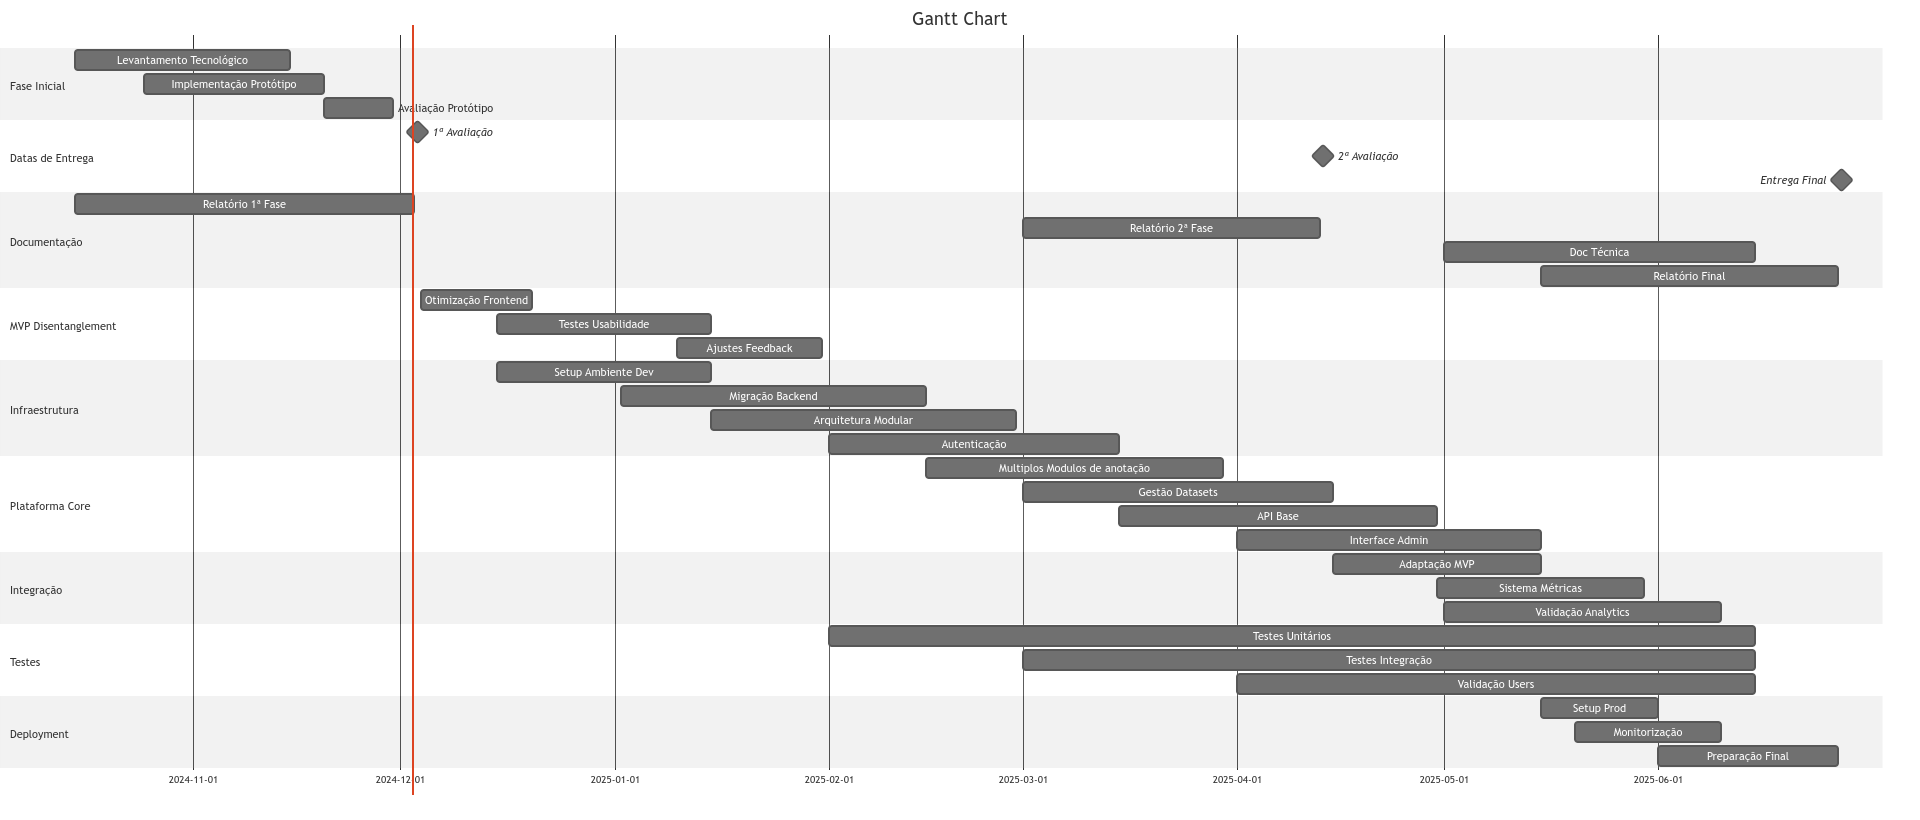
\includegraphics[width=0.98666\paperheight, angle=0, keepaspectratio]{images/Gant.drawio.png}
        }
        \caption{Cronograma detalhado do projeto (Gantt Chart) - Estado Atualizado}
        \label{fig:gantt-chart}
    \end{figure}
\end{landscape}

    \chapter{Resultados}

% Este capítulo será desenvolvido nas fases posteriores do projeto,
% quando houver resultados concretos para apresentar.

    \chapter{Conclusão}

% A conclusão será desenvolvida na fase final do projeto,
% apresentando uma análise completa dos resultados obtidos.

    
    % Appendices
    \appendix
    %\input{appendices/(recomendacoes-formatacao)}
    %\input{appendices/(documentacao-tecnica)}
    %\input{appendices/(prototipos-detalhados)}
    
    \clearpage
    \addcontentsline{toc}{chapter}{Referências Bibliográficas}
    \printbibliography[title={Referências Bibliográficas}]
    \printglossary[title=Glossário,toctitle=Glossário]
\end{document}
